\documentclass{article}
\usepackage{../../Self_Style}

\title{Phys 115A HW 3}
\author{Zih-Yu Hsieh}
\date{\today}

\begin{document}
\maketitle

\section*{1}
\begin{ques}\label{q1}
\textbf{Clever Commutation}

Suppose I give you a quantum system that can be described with a raising operator $a^+$ and
a lowering operator $a^-$ that satisfy the commutation relation $[a^-, a^+] = 1$ (it doesn’t have
to be the quantum harmonic oscillator, specifically). You know that there is a properly-
normalized state $\psi$ that is annihilated by $a^-$, i.e., you know that $a^- \psi = 0$, but I don’t tell
you how $a^+$ acts on $\psi$.

(a) I prepare for you a state
\[
\Psi = c\times (a^-a^-a^-a^-a^+a^+a^+a^+\psi)
\]
where $c$ is a real constant. Is $\Psi$ a normalizable state? If so, find $c$ such that $\Psi$ is
properly normalized. What is the relation between $\Psi$ and $\psi$?

(b) I prepare for you a different state
\[
\Psi = c\times (a^-a^-a^-a^-a^+a^+ \psi)
\]
where $c$ is a real constant. Is this new $\Psi$ a normalizable state? If so, find $c$ such that
$\Psi$ is properly normalized.
\end{ques}

\begin{proof}

    \hfil

    \begin{itemize}
        \item[(a)] Given that $[a^-, a^+]=1$ (or identity operator), we have $a^-a^+=1+a^+a^-$, so the relation $a^-a^+\psi=\psi+a^+a^-\psi = \psi$, hence $\psi$ is an eigenvector of the linear operator $a^-a^+$ with eigenvalue $1$. Which, if consider the vector $a^+\psi$, we get the following:
        \begin{align}
            a^-a^+(a^+\psi) &= a^+\psi+a^+(a^-a^+\psi) = a^+\psi + a^+\psi=2(a^+\psi)
        \end{align}
        Hence, $a^+\psi$ is an eigenvector of $a^-a^+$ with eigenvalue $2$. Inductively, suppose given $n\in\NN$ one has $(a^+)^n\psi$ being an eigenvector of $a^-a^+$ with eigenvalue $(n+1)$, then for the case of $(n+1)$, the following is true:
        \begin{align}
            a^-a^+((a^+)^{n+1}\psi) &= (a^+)^{n+1}\psi+a^+(a^-(a^+)^{n+1}\psi)=(a^+)^{n+1}\psi+a^+((a^-a^+)(a^+)^{n}\psi)\\
            &= (a^+)^{n+1}\psi+(n+1) a^+(a^+)^{n}\psi = (n+2)(a^+)^{n+1}\psi
        \end{align}
        Hence, by induction, all $n\in\NN$ satisfies $(a^+)^n\psi$ being an eigenvector of $a^-a^+$ with eigenvalue $(n+1)$.

        With some simplification, another round of induction can be done on the vector of the form $\Psi=(a^-)^n(a^+)^n\psi$: For $n=2$, one has $(a^-)(a^-a^+)(a^+\psi) = 2a^-a^+\psi = 2\psi$. Which, inductively suppose given $n\in\NN$ one has $(a^-)^n(a^+)^n\psi=n!\psi$, then for the case of $(n+1)$, the following is true:
        \begin{align}
            (a^-)^{n+1}(a^+)^{n+1}\psi &= (a^-)^n (a^-a^+)(a^+)^n\psi = (n+1)(a^-)^n(a^+)^n \psi = (n+1)!\psi
        \end{align}
        Hence, by induction, all $n\in\NN$ satisfies $(a^-)^n(a^+)^n\psi = n!\psi$. So, with $\Psi = c(a^-)^4(a^+)^4\psi$, one has $\Psi = c\cdot 4!\psi$, hence with $c!=0$, $\Psi$ (viewed as a state) is normalizable. With $\psi$ being normalized, it requires $c=\frac{1}{4!}$ for $\Psi$ to be properly normalized.

        \hfil

        \item[(b)] Adapt the machinery built in part (a), given $\Psi=c(a^-)^4(a^+)^2\psi = c(a^-)^2((a^-)^2(a^+)^2\psi)$, it reduces to $\Psi = c(a^-)^2(2!\psi) = 0$ (since $a^-\psi=0$). Hence, $\Psi$ is the zero-vector, which is not normalizable.
    \end{itemize}

\end{proof}

\hfil

\section*{2 (ND, remark (d), calculate (e))}
\begin{ques}\label{q2}
\textbf{Constructing States (modified Griffiths 2.10 and 2.14)}

Given the explicit solution for the ground state of the harmonic oscillator,
\[
\psi_0(x) = \left(\frac{m\omega}{\pi \hbar}\right)^{1/4} e^{- \frac{m\omega}{2\hbar}x^2}
\]

(a) Construct $\psi_2(x)$ explicitly using the algebra formalism. (Hint: $\psi_1(x)$ is constructed
this way in Griffiths Example 2.4.)

(b) Check the orthogonality of $\psi_0$, $\psi_1$, and $\psi_2$ by explicit integration. Hint: If you exploit
the evenness and oddness of the functions, there is really only one integral left to
do.

(c) Find the classical turning points for $\psi_0$, $\psi_1$, and $\psi_2$ (i.e., the values of $x$ where the
kinetic energy goes to zero for a classical harmonic oscillator of known total energy).

(d) Sketch $\psi_0$, $\psi_1$, $\psi_2$, $\psi_3$. For each state, mark the classical turning point. How does the
classical turning point relate to the form of the wavefunction?

(e) For $\psi_0$, what is the probability (correct to three significant digits) of finding the
particle outside the classically allowed region, meaning outside the classical turning
points? You can use a math table under “Normal Distribution” or Mathematica or
any other tool you wish to numerically evaluate the relevant integral.
\end{ques}

\begin{proof}
    For this question, recall the definition of the operators: $a_\pm = \frac{1}{\sqrt{2\hbar mw}}(mw\hat{x} \mp i\hat{p})$, $\hat{x}$ is the operator simply by multiplying $x$, and $\hat{p}=\frac{\hbar}{i}\frac{\partial}{\partial x}$. So, $a_\pm = \frac{1}{\sqrt{2\hbar mw}}(mwx \mp \hbar\frac{\partial}{\partial x})$.

    \begin{itemize}
        \item[(a)] Recall that $\psi_n(x) = \frac{1}{\sqrt{n!}}(a_+)^n \psi_0(x)$. So, for $n=2$,  one derives the following:
        \begin{align}
            a_+ \psi_0(x)&=\frac{1}{\sqrt{2\hbar mw}}\left(mwx - \hbar\frac{\partial}{\partial x}\right)\left(
            \left(\frac{mw}{\pi \hbar}\right)^\frac{1}{4}e^{-\frac{mw}{2\hbar}x^2}\right) \\
            &= \sqrt{\frac{mw}{2\hbar}}\left(\frac{mw}{\pi\hbar}\right)^\frac{1}{4}xe^{-\frac{mw}{2\hbar}x^2} + \sqrt{\frac{\hbar}{2mw}}\left(\frac{mw}{\pi\hbar}\right)^\frac{1}{4}\frac{mw}{\hbar}xe^{-\frac{mw}{2\hbar}x^2}\\
            &= 2\sqrt{\frac{mw}{2\hbar}}\left(\frac{mw}{\pi\hbar}\right)^\frac{1}{4}xe^{-\frac{mw}{2\hbar}x^2} = \sqrt{\frac{2mw}{\hbar}}\left(\frac{mw}{\pi\hbar}\right)^\frac{1}{4}xe^{-\frac{mw}{2\hbar}x^2}
        \end{align}
        \begin{align}
            (a_+)^2\psi_0(x)& = \frac{1}{\sqrt{2\hbar mw}}\left(mwx - \hbar\frac{\partial}{\partial x}\right)\left(\sqrt{\frac{2mw}{\hbar}}\left(\frac{mw}{\pi\hbar}\right)^\frac{1}{4}xe^{-\frac{mw}{2\hbar}x^2}\right)\\
            &= \frac{mw}{\hbar}\left(\frac{mw}{\pi\hbar}\right)^\frac{1}{4}x^2e^{-\frac{mw}{2\hbar}x^2} - \left(\frac{mw}{\pi\hbar}\right)^\frac{1}{4}e^{-\frac{mw}{2\hbar}x^2} + \left(\frac{mw}{\pi\hbar}\right)^\frac{1}{4}\cdot \frac{mw}{\hbar}x^2e^{-\frac{mw}{2\hbar}x^2}\\
            &= \frac{2mw}{\hbar}\left(\frac{mw}{\pi\hbar}\right)^\frac{1}{4}x^2e^{-\frac{mw}{2\hbar}x^2} - \left(\frac{mw}{\pi\hbar}\right)^\frac{1}{4}e^{-\frac{mw}{2\hbar}x^2}
        \end{align}
        So, we get that $\psi_2(x)=\frac{1}{\sqrt{2}}(a_+)^2\psi_0(x) = \frac{\sqrt{2}mw}{\hbar}\left(\frac{mw}{\pi\hbar}\right)^\frac{1}{4}x^2e^{-\frac{mw}{2\hbar}x^2} - \frac{1}{\sqrt{2}}\left(\frac{mw}{\pi\hbar}\right)^\frac{1}{4}e^{-\frac{mw}{2\hbar}x^2}$.

        \hfill

        \item[(b)] It suffices to check orthogonality for $\psi_0, (a_+)\psi_0, (a_+)^2\psi_0$ (since scaling doesn't affect orthogonality). 

        For $\psi_0, (a_+)\psi_0$, the integration provides the following:
        \begin{align}
            \int_{-\infty}^{\infty}((a_+)\psi_0(x))^* \psi_0(x)dx= \int_{-\infty}^{\infty}\sqrt{\frac{2mw}{\hbar}}\left(\frac{mw}{\pi\hbar}\right)^\frac{1}{4}xe^{-\frac{mw}{2\hbar}x^2}\cdot \left(\frac{m\omega}{\pi \hbar}\right)^{1/4} e^{- \frac{m\omega}{2\hbar}x^2}dx=0
        \end{align}
        (Note: The above is an integration of an odd function that converges, hence provides $0$). Hence, $\psi_0, (a_+)\psi_0$ are orthogonal under integration of inner product.

        For $(a_+)\psi_0, (a_+)^2\psi_0$, the integration provides the following:
        \begin{align}
            &\int_{-\infty}^{\infty}((a_+)\psi_0(x))^* ((a_+)^2\psi_0(x))dx\\
            &= \int_{-\infty}^{\infty}\sqrt{\frac{2mw}{\hbar}}\left(\frac{mw}{\pi\hbar}\right)^\frac{1}{4}xe^{-\frac{mw}{2\hbar}x^2}\cdot \left(\frac{\sqrt{2}mw}{\hbar}\left(\frac{mw}{\pi\hbar}\right)^\frac{1}{4}x^2e^{-\frac{mw}{2\hbar}x^2} - \left(\frac{mw}{\pi\hbar}\right)^\frac{1}{4}e^{-\frac{mw}{2\hbar}x^2}\right)dx\\
            &= K\int_{-\infty}^{\infty}x^3e^{-\frac{mw}{\hbar}x^2}dx + L\int_{-\infty}^{\infty}xe^{-\frac{mw}{\hbar}x^2}dx = 0
        \end{align}
        (Note: Above are two odd function that has converging integrals, which with domain being symmetric it converges to $0$. $K,L$ are proper substitutions of the constants).
        Hence, $(a_+)\psi_0, (a_+)^2 \psi_0$ are also orthogonal under integration inner product.

        Finally, for $\psi_0, (a_+)^2\psi_0$, the integration provides the following:
        \begin{align}
            &\int_{-\infty}^{\infty}(\psi_0(x))^*((a_+)^2\psi_0(x))dx\\
            &= \int_{-\infty}^{\infty}\left(\frac{m\omega}{\pi \hbar}\right)^{1/4} e^{- \frac{m\omega}{2\hbar}x^2}\left(\frac{\sqrt{2}mw}{\hbar}\left(\frac{mw}{\pi\hbar}\right)^\frac{1}{4}x^2e^{-\frac{mw}{2\hbar}x^2} - \frac{1}{\sqrt{2}}\left(\frac{mw}{\pi\hbar}\right)^\frac{1}{4}e^{-\frac{mw}{2\hbar}x^2}\right) dx\\
            &= -\frac{1}{\sqrt{2}}\int_{-\infty}^{\infty}\sqrt{\frac{mw}{\pi\hbar}}e^{-\left(\sqrt{\frac{mw}{\hbar}}x\right)^2}dx + \frac{\sqrt{2}mw}{\hbar}\int_{-\infty}^{\infty}\sqrt{\frac{mw}{\pi \hbar}}x^2 e^{-\frac{mw}{\hbar}x^2}dx\\
            &= -\frac{1}{\sqrt{2}} - \frac{\sqrt{2}mw}{\hbar}\left(\int_{-\infty}^{\infty}\sqrt{\frac{mw}{\pi \hbar}}\frac{\partial}{\partial \lambda}\left(e^{-\lambda x^2}\right)dx\right) \bigg|_{\lambda=\frac{mw}{\hbar}}\\
            &= -\frac{\sqrt{2}mw}{\hbar}\frac{d}{d\lambda}\bigg|_{\lambda=\frac{mw}{\hbar}}\int_{-\infty}^{\infty}\sqrt{\frac{mw}{\pi\hbar}}e^{-\lambda x^2}dx - \frac{1}{\sqrt{2}} = -\frac{\sqrt{2}mw}{\hbar}\sqrt{\frac{mw}{\pi\hbar}}\sqrt{\frac{\pi}{\lambda}}\bigg|_{\lambda=\frac{mw}{\hbar}} - \frac{1}{\sqrt{2}}\\
            &= -\sqrt{\frac{2}{\pi}}\left(\frac{mw}{\hbar}\right)^\frac{3}{2}\cdot\left(-\frac{1}{2}\frac{\sqrt{\pi}}{\lambda^\frac{3}{2}}\right)\bigg|_{\lambda=\frac{mw}{\hbar}} - \frac{1}{\sqrt{2}} = \frac{1}{\sqrt{2}}-\frac{1}{\sqrt{2}}=0
        \end{align}
        Hence, under integration inner product, $\psi_0, (a_+)^2\psi_0$ are also orthogonal.

        Since $\psi_0,\psi_1,\psi_2$ are scalar multiples of $\psi_0,(a_+)\psi_0,(a_+)^2\psi_0$ respectively, hence they're also mutually othogonal under integration inner product.

        \hfill

        \item[(c)] Given the energy of $\psi_n(x)$ is $E_n=\left(n+\frac{1}{2}\right)\hbar w$, and the potential energy is $V(x)=\frac{1}{2}mw^2 x^2$, the classical turning points occurs when $E_n=V(x)$, providing the following solution:
        \begin{align}
            \frac{1}{2}mw^2 x^2=\left(n+\frac{1}{2}\right)\hbar w \implies x = \pm\sqrt{\left(n+\frac{1}{2}\right)\frac{2\hbar}{mw}} = \pm\sqrt{\frac{(2n+1)\hbar}{mw}}
        \end{align}
        Hence, the classical turning points of the four states $\psi_0,\psi_1,\psi_2$ (denoted as $\pm x_0, \pm x_1, \pm x_2$ respectively) are given as:
        \begin{align}
            \pm x_0 = \pm\sqrt{\frac{\hbar}{mw}},\quad \pm x_1=\pm\sqrt{\frac{3\hbar}{mw}},\quad \pm x_2=\pm\sqrt{\frac{5\hbar}{mw}}
        \end{align}

        \hfill

        \item[(d)] Here are some graphs of the first four states (starting from ground states):
        
        \begin{figure}[th!]
            \centering
            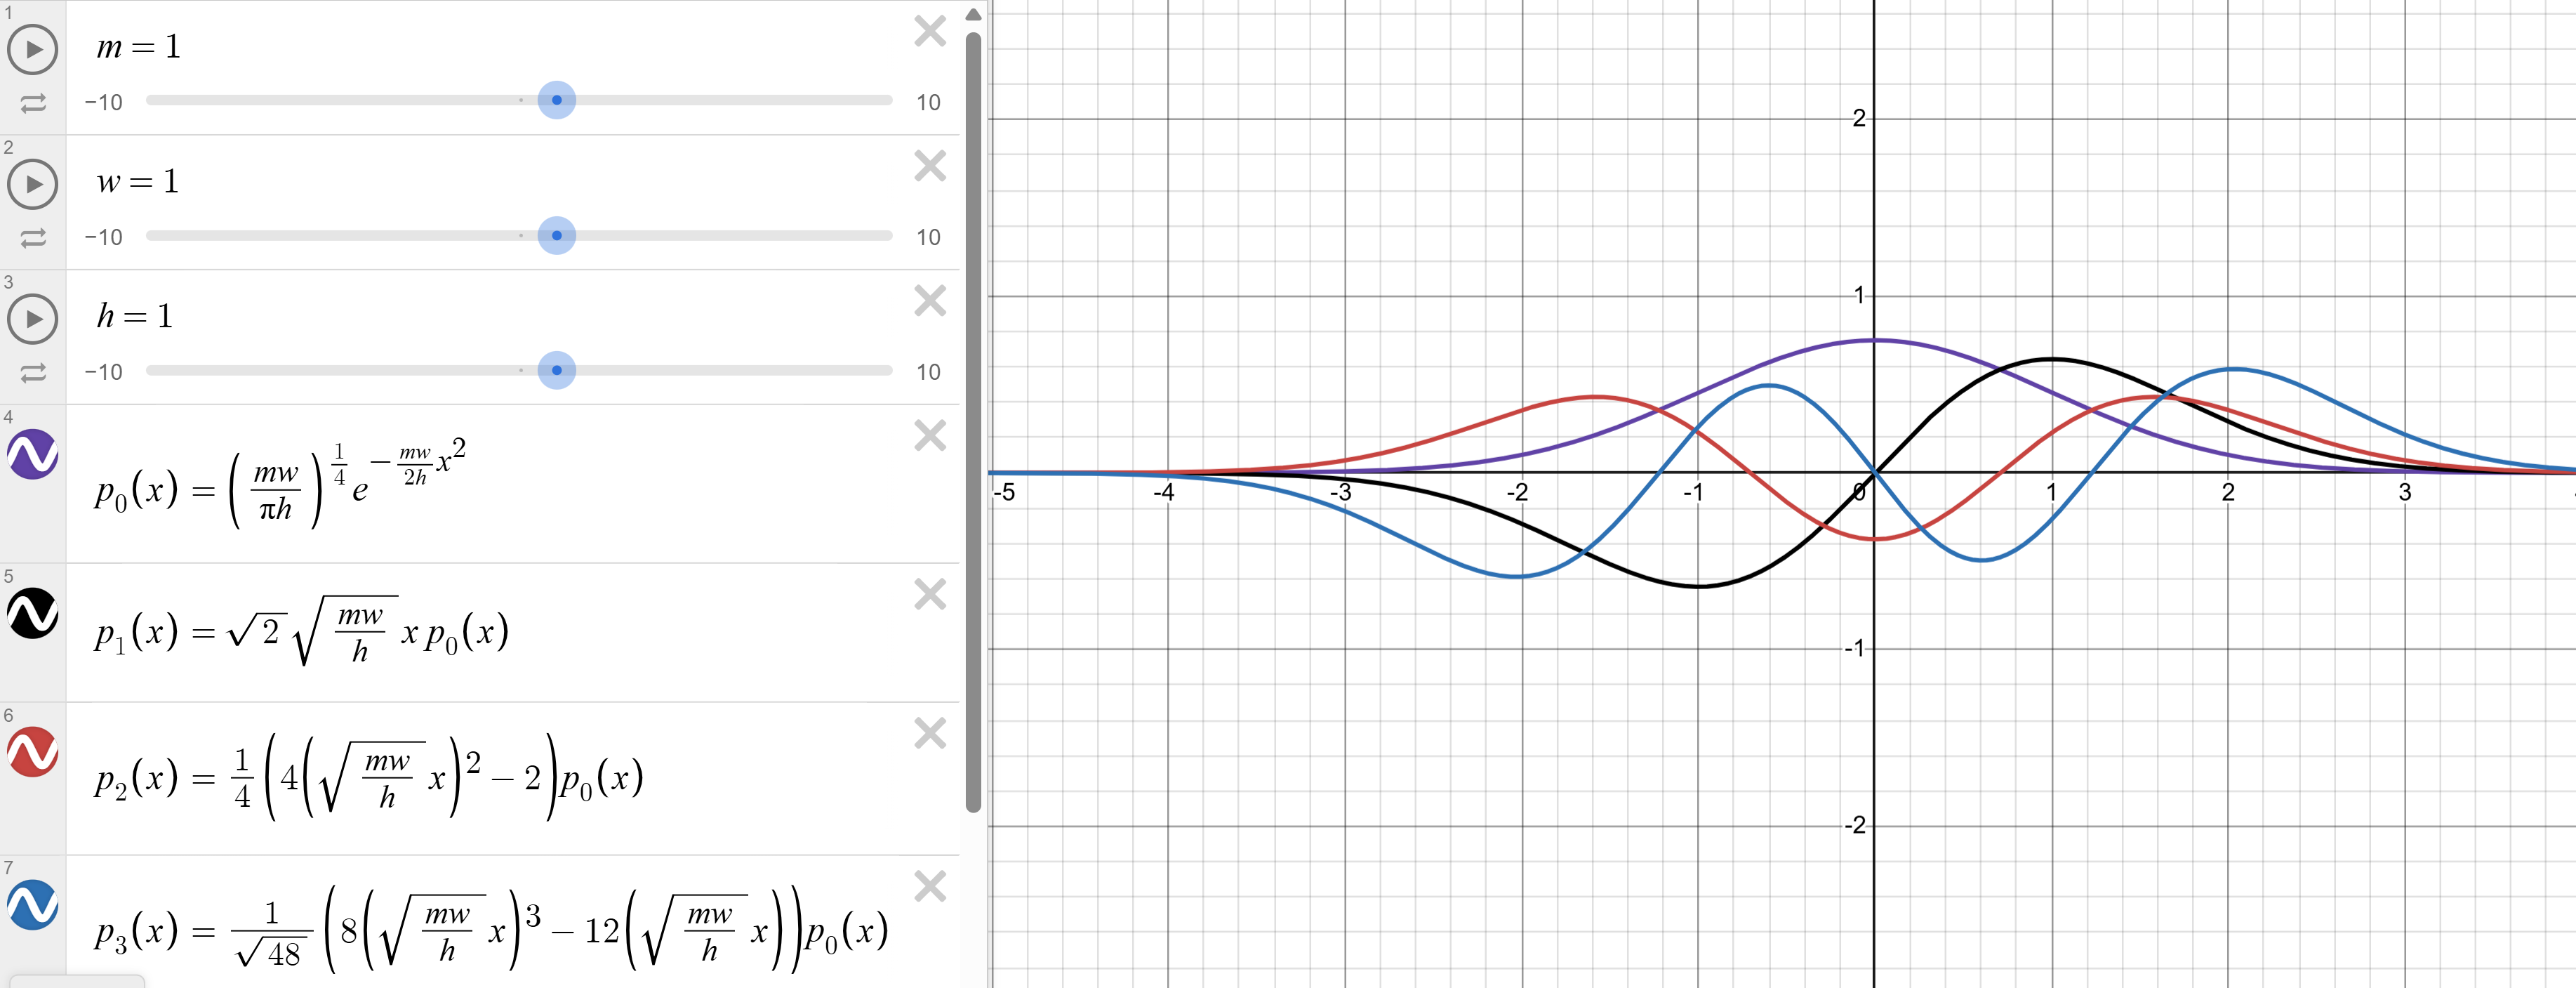
\includegraphics[width=150mm]{oscillator_sketch.png}
        \end{figure}

        Here, the classical turning point actually represents the farthest positions from the origin where the second derivative of the wavefunction is $0$ (or the farthest point the wave function changes its concavity).

        \hfil

        \item[(e)] Recall that from part (d), the classical turning point
        
    \end{itemize}
\end{proof}

\newpage

\section*{3 (ND, tweak constants in (a))}
\begin{ques}\label{q3}
\textbf{Uncertainty Principle for the nth state (modified Griffiths 2.12)}

Consider the $n$th stationary state of the harmonic oscillator.

(a) Find $\langle x \rangle$, $\langle p \rangle$, $\langle x^2 \rangle$ and $\langle p^2 \rangle$ for this state, following the method of Example 2.5.

(b) Find the expectation value of the kinetic energy, $\langle T \rangle$, and the expectation value of
the potential energy, $\langle V \rangle$, for this state.

(c) Compute $\sigma_x \sigma_p$ for this state, and check that the uncertainty principle is satisfied.
Under what circumstances is it saturated (i.e., is $\sigma_x \sigma_p = \hbar/2$)?

Hint: For this problem, do not explicitly integrate the wavefunction, which has a terrible
form for arbitrary $n$. Instead, notice that you can write $x$ and $p$ in terms of raising and
lowering operators,
\[
x = \sqrt{\frac{\hbar}{2m\omega}} (a^+ + a^-), \quad
p = i\sqrt{\frac{\hbar m\omega}{2}} (a^+ - a^-).
\]
Then to compute the expectation values you just have to act on $\psi_n$ with raising and
lowering operators, which you know how to do.
\end{ques}

\begin{proof}

    Here, we'll assume the fact that the list $\{\psi_n\}_{n\in\NN}$ forms an orthonormal list under integration inner product (so, for $n\neq m$, it satisfies $\int_{-\infty}^{\infty}\psi_n(x)^*\psi_m(x)dx=0$). Also, we'll utilize the fact that $a^+,a^-$ are Adjoint Operators/Hermition Conjugates of each other, which implies that $\int_{-\infty}^{\infty}\psi(x)^* (a^+\phi(x))dx=\int_{-\infty}^{\infty}(a^-\psi(x))^* \phi(x)dx$, and $\int_{-\infty}^{\infty}\psi(x)^* (a^-\phi(x))dx=\int_{-\infty}^{\infty}(a^+\psi(x))^* \phi(x)dx$.

    Also, based on these rule, let $T^*$ denote the adjoint / Hermitian Conjugate of linear operator $T$, then we get that $\hat{p}^* = -i\sqrt{\frac{\hbar mw}{2}}((a^+)^*-(a^-)^*) = -i\sqrt{\frac{\hbar mw}{2}}(a^--a^+) = i\sqrt{\frac{\hbar m\omega}{2}} (a^+ - a^-) = \hat{p}$.

    \begin{itemize}
        \item[(a)] Given $\psi_n(x)=(a^+)^n\psi_0(x)$, using the expression that $\hat{x}=\sqrt{\frac{\hbar}{2mw}}(a^++a^-)$ as operator, we get the following (where below is up to some constant):
        \begin{align}
            \left<x\right>&=\int_{-\infty}^{\infty}\psi_n(x)^* (\hat{x}\psi_n(x))dx = \sqrt{\frac{\hbar}{2mw}}\int_{-\infty}^{\infty}((a^+)^n \psi_0(x))^*((a_+)^{n+1}\psi_0(x)+a^- (a^+)^n\psi_0(x))dx\\
            &= \sqrt{\frac{\hbar}{2mw}}\int_{-\infty}^{\infty}\psi_n(x)^* \psi_{n+1}(x)dx + \sqrt{\frac{\hbar}{2mw}}\int_{-\infty}^{\infty}((a^+)^n\psi_0(x))^* a^-((a^+)^n\psi_0(x))dx\\
            &= 0+\sqrt{\frac{\hbar}{2mw}}\int_{-\infty}^{\infty}((a^+)^{n+1}\psi_0(x))^* \psi_n(x)dx = \sqrt{\frac{\hbar}{2mw}}\int_{-\infty}^{\infty}\psi_{n+1}(x)^*\psi_n(x)dx = 0
        \end{align}
        \begin{align}
            \left<p\right>&=\int_{-\infty}^{\infty}\psi_n(x)^*(\hat{p}\psi_n(x))dx = i\sqrt{\frac{\hbar mw}{2}}\int_{-\infty}^{\infty}((a^+)^n\psi_0(x))^*((a^+)^{n+1}\psi_0(x)-a^-(a^+)^{n}\psi_0(x))dx\\
            &= i\sqrt{\frac{\hbar mw}{2}}\left(\int_{-\infty}^{\infty}\psi_n(x)^* \psi_{n+1}(x)dx - \int_{-\infty}^{\infty}((a^+)^{n+1}\psi_0(x))^*((a^+)^n \psi_0(x))dx\right)\\
            &= 0-i\sqrt{\frac{\hbar mw}{2}}\int_{-\infty}^{\infty}\psi_{n+1}(x)^* \psi_n(x)dx = 0
        \end{align}
        \begin{align}
            \left<x^2\right> &= \int_{-\infty}^{\infty}\psi_n(x)^2 x^2 \psi_n(x)dx = \int_{-\infty}^{\infty}(\hat{x}\psi_n(x))^*(\hat{x}\psi_n(x))dx\\
            &= \frac{\hbar}{2mw}\int_{-\infty}^{\infty}((a^+)^{n+1}\psi_0(x) + a^-(a^+)^n\psi_0(x))^* ((a^+)^{n+1}\psi_0(x) + a^-(a^+)^n\psi_0(x))dx\\
            &= \frac{\hbar}{2mw}\int_{-\infty}^{\infty}(\sqrt{(n+1)!}\psi_{n+1}(x)+\sqrt{n!}\psi_{n-1}(x))^*(\sqrt{(n+1)!}\psi_{n+1}(x)+\sqrt{n!}\psi_{n-1}(x))dx\\
            &= \frac{\hbar}{2mw}((n+1)!+n!)
        \end{align}
        (Note: the last equality is using the fact that the integration represents the $\|\sqrt{(n+1)!}\psi_{n+1}(x)+\sqrt{n!}\psi_{n-1}(x)\|^2$, by orthonormality and Pythagoreus Theorem of inner product, such norm is the same as $\|\sqrt{(n+1)!}\|\psi_{n+1}(x)\|^2+\|\sqrt{n!}\psi_{n-1}(x)\|^2 = (n+1)!+n!$).
        \begin{align}
            \left<p^2\right> &= \int_{-\infty}^{\infty}\psi_n(x)^*(\hat{p}^2 \psi_n(x))dx = \int_{-\infty}^{\infty}(\hat{p}\psi_n(x))^*(\hat{p}\psi_n(x))dx\\
            &= \frac{\hbar mw}{2}\int_{-\infty}^{\infty}(a^+\psi_n(x)-a^-\psi_n(x))^*(a^+\psi_n(x)-a^-\psi_n(x))dx\\
            &= \frac{\hbar mw}{2}(2n+1)
        \end{align} (check the precise statement about how $a^+,a^-$ acts on $\psi_n(x)$ with constant).

        \hfil

        \item[(b)]Kinetic energy $\hat{T}:=\frac{\hat{p}^2}{2m}$, hence $\left<T\right>=\int_{-\infty}^{\infty}\psi_n(x)^* (\frac{\hat{p}^2}{2m}\psi_n(x))dx = \frac{\left<p^2\right>}{2m}$.
        
        Similarly, given potential energy $V(x)=\frac{1}{2}mw^2 x^2$, then $\left<V\right>=\int_{-\infty}^{\infty}\psi_n(x)^* (\frac{1}{2}mw^2 x^2\psi_n(x))dx = \frac{1}{2}mw^2 \left<x^2\right>$.

        \hfil

        \item[(c)] Need to wait until the constants in (a) is checked.
    \end{itemize}
\end{proof}

\newpage

\section*{4 (ND)}
\begin{ques}\label{q4}
\textbf{Back of the envelope}

Using the symmetry of the potential, come up with an expression for the zero-point energy
of a harmonic oscillator on the assumption that it is the minimum energy required by the
uncertainty principle.
\end{ques}

\begin{proof}
\end{proof}

\newpage

\section*{5 (ND)}
\begin{ques}\label{q5}
\textbf{Coherent states}

In problem 3, you found that most of the stationary states of the harmonic oscillator satisfy,
but do not saturate, the uncertainty principle. Now let us consider a special superposition of
these stationary states called a coherent state, which has some fairly interesting properties.
We call such a state an eigenfunction of the lowering operator. It just means the coherent
state $S_\alpha(x)$ satisfies $a^- S_\alpha(x) = \alpha S_\alpha(x)$ where $\alpha$ is a complex number.
Note that there are no normalizable eigenfunctions of the raising operator.

(a) Calculate $\langle x \rangle$ and $\langle p \rangle$ for the state $S_\alpha(x)$. Does this remind you of anything from
previous problems in this set? Hint: Since you know how $a^-$ acts on $S_\alpha(x)$, use the
fact that
\[
\int_{-\infty}^{\infty} f^*(x)(a^\pm g(x))\,dx
= \int_{-\infty}^{\infty} (a^\mp f(x))^* g(x)\,dx.
\]
Also, keep in mind that $\alpha$ is in general complex.

(b) Calculate $\langle x^2 \rangle$ and $\langle p^2 \rangle$ for the state $S_\alpha(x)$.

(c) Show that $S_\alpha$ saturates the uncertainty principle.

(d) We can express $S_\alpha(x)$ at $t = 0$ explicitly in terms of the stationary states $\psi_n$,
\[
S_\alpha(x) = \sum_{n=0}^{\infty} c_n \psi_n(x)
\]
Show that $c_n = \frac{\alpha^n}{\sqrt{n!}} c_0$. Hint: Keep using the earlier hint!

(e) Fix $c_0$ by normalizing $S_\alpha(x)$.

(f) Now consider $S_\alpha(x, t)$,
\[
S_\alpha(x, t) = \sum_{n=0}^{\infty} c_n \psi_n(x)e^{-iE_n t/\hbar}.
\]
Show that $S_\alpha(x, t)$ remains an eigenfunction of $a^-$ but that $\alpha$ now evolves in time.
That is, show that $a^- S_\alpha(x, t) = \alpha(t) S_\alpha(x, t)$, where $\alpha(t) = e^{-i\omega t}\alpha$.
Argue that this means coherent states stay coherent in time, and continue to saturate the
uncertainty principle.

(g) Can we think of the ground state $\psi_0$ as a coherent state? What is $\alpha$ in this case?

These states are profoundly interesting in quantum optics, since they provide an accurate
quantum description of laser light. Roy Glauber was awarded half of the Nobel Prize in
Physics in 2005 for his 1963 work on understanding the properties of coherent states in
quantum optics.
\end{ques}

\begin{proof}
\end{proof}

\newpage

\end{document}